\section{Architecture}
Architecture contains main server which serves data to clients (in this case users equipped with web browsers). Then it communicate with backend servers through RESTful API to get data for clients.

In addition main server is an entity which can represent multiple servers hidden behind load balancer for scaling for high load plus one additional server for storing database and shared files via NFS\@.

\begin{figure}[!htbp]
\centering
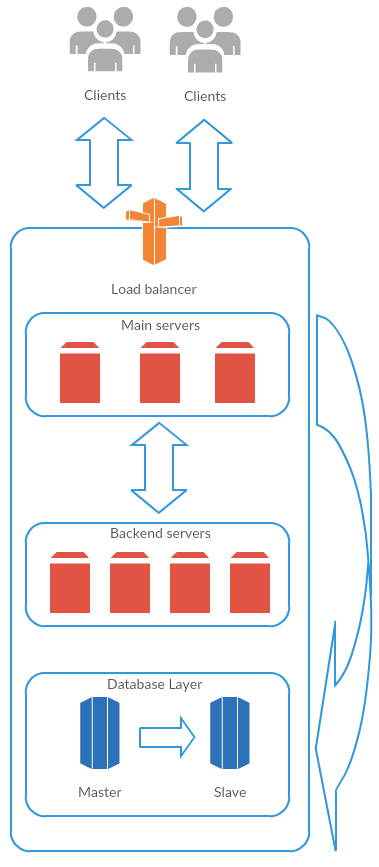
\includegraphics[scale=0.5]{architecture}
\label{fig:architecture}
\caption{Architecture of the whole system}
\end{figure}

\section{Framework design}
For the purpose of implementing aforementioned architecture a framework was created in new language ``Go'' backed by Google\cite{Go-wiki}. It can be further reused in other projects as it was released as a Free Software. The choice of Go as a language is not accidental. It has a really well defined standard library and it is very secure statically typed language with no implicit types conversions. Not to mentioned that is really fast in execution, but as a drawback writing a code feels really verbose.

Framework uses middlewares for modifying every new request and then response that is sent to a user. For instance we can create middleware purely for authentication process. If the user malformed credentials then middleware will modify the response so that the user knows that he provided them wrong.

\begin{figure}[!htbp]
\centering
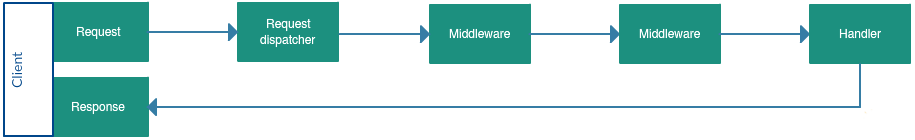
\includegraphics[scale=0.45]{middleware}
\caption[Request flow through middlewares]{Request flow through middlewares. Note that each middleware can modify request and response as they wish.}
\label{fig:middleware}
\end{figure}

\section{Authentication system}
Authentication system is implemented as middleware and uses standarized JWT tokens\cite{JWT-rfc}. The big benefit is that we do not need to store session in our database, we only need to verify that the token was signed by us.

\section{Security}
The security is implemented at different levels. Connection is secured by standard TLS/SSL on HTTP level. Some resources require user to be authenticated (valid token).
